% !TeX TXS-program:compile = txs:///xelatex/[--shell-escape]
% IACR Transactions CLASS DOCUMENTATION
% Written by Gaetan Leurent gaetan.leurent@inria.fr (2016-2018)
%
% To the extent possible under law, the author(s) have dedicated all
% copyright and related and neighboring rights to this software to the
% public domain worldwide. This software is distributed without any
% warranty.
%
% You should have received a copy of the CC0 Public Domain Dedication
% along with this software. If not, see
% <http://creativecommons.org/publicdomain/zero/1.0/>.

\documentclass[preprint]{iacrtrans}
\usepackage[utf8]{inputenc}

\setcounter{tocdepth}{4}

%% VERSION
\newcommand{\version}{v.1.0}


%% TITLE
\title{
  
\includegraphics[width=\columnwidth]{logo_zkEVM.png} \\ \vspace{0.3cm}
  From Zero to zkEVM - Communication Layer \vspace{0.3cm}\\
  \version
}

\institute{}


\usepackage{caption}
\usepackage{subcaption}

% This package controls how hyperlinks are displayed
% https://es.overleaf.com/learn/latex/Hyperlinks
\usepackage{hyperref}
\hypersetup{colorlinks=true,linkcolor={red!80!black},urlcolor={blue!80!black}}

%Multiple columns
\usepackage{multicol}

% Used for super caligraphic font \mathscr{}
\usepackage{mathrsfs}

%This ensures spaces when using ensuremath and no $$ are used to introduce math
\usepackage{xspace}

%%%%%% BEGIN OF CODE HIGHLIGHTING ENVIRONMENTS %%%%%%

%   sudo apt install texlive-latex-extra
%   sudo apt install python-pip
%   pip install pygments
%   pip install pygments-lexer-babylon  #contains JSX
%   pip install pygments-lexer-solidity
%   pip install pygments pygments-lexer-babylon pygments-lexer-solidity


% *** COLOR COMMANDS ***
\definecolor{dblackcolor}{rgb}{0.0,0.0,0.0}
\definecolor{dbluecolor}{rgb}{0.01,0.02,0.5}
\definecolor{dgreencolor}{rgb}{0.2,0.4,0.0}
\definecolor{dgraycolor}{rgb}{0.30,0.3,0.30}
\newcommand{\dblue}{\color{dbluecolor}\bf}
\newcommand{\dred}{\color{dredcolor}\bf}
\newcommand{\dblack}{\color{dblackcolor}\bf}
\definecolor{light-gray}{gray}{0.96} %the shade of grey that stack exchange uses

\usepackage{showexpl}% already includes listings package
\makeatletter
\def\lst@filenamerpl{_\textunderscore $\textdollar}
\makeatother
\lstset{frame=shadowbox, basicstyle=\footnotesize\ttfamily, showstringspaces=false,
rulesepcolor=\color{black}, upquote=true}

\lstdefinestyle{scriptStyle}{
    basicstyle=\footnotesize,% control font of code
    preset=\footnotesize,% adjust font size of output
    numbers=none,
    frame=tlbr,
    pos=r,% want output on rightbackgroundcolor=\color{yellow!30},
    width=0.50\linewidth,
}

\lstdefinestyle{terms}{
    basicstyle=\scriptsize\ttfamily,% control font of code
    preset=\footnotesize,% adjust font size of output
}

\lstdefinestyle{termt}{
    basicstyle=\footnotesize\ttfamily,% control font of code
    preset=\footnotesize,% adjust font size of output
	numbers=none,
}

\lstdefinestyle{verb}{
    basicstyle=\footnotesize,% control font of code
    preset=\footnotesize,% adjust font size of output
    frame=tlbr,
    pos=r,% want output on right
%     backgroundcolor=\color{yellow!30},
    width=0.50\linewidth,
}

\lstdefinestyle{verbs}{
    basicstyle=\scriptsize,% control font of code
    preset=\scriptsize,% adjust font size of output
    frame=tlbr,
    pos=r,% want output on right
%     backgroundcolor=\color{yellow!30},
    width=0.50\linewidth,
}

\lstdefinestyle{verbt}{
    basicstyle=\tiny\ttfamily,% control font of code
    preset=\tiny\ttfamily,% adjust font size of output
    frame=tlbr,
    pos=r,% want output on right
%     backgroundcolor=\color{yellow!30},
    width=0.50\linewidth,
}

%Linter for circom
\usepackage{tcolorbox}
\tcbuselibrary{minted,skins,listings}
\definecolor{mybg}{rgb}{0.96,0.96,0.98}
% \lstset{
% 	backgroundcolor = \color{light-gray},
% 	showtabs = False,
% 	tabsize = 2,
% 	showspaces = False,
% 	showstringspaces = False,
% 	commentstyle = {\ttfamily\color{dgreencolor}},
% 	keywordstyle = {\ttfamily\color{dbluecolor}\bfseries},
% 	stringstyle = {\ttfamily\color{dgraycolor}\bfseries},
% 	language = circom,
% 	basicstyle = {\fontsize{7pt}{7pt}\ttfamily},
% 	aboveskip = 1em,
% 	belowskip = 1em,
% 	numbers = left,%none,
% 	numbersep=5pt,    %space line numbers from code
% 	xleftmargin=2em,
% 	frame=single,	% adds a frame around the code
% 	framexleftmargin=1.7em,
% 	numberstyle=\tiny,%\color{gray}
% 	emph = {proc,retp,endp,local},
% 	emphstyle = {\color{blue}\textbf},
% 	literate =
% 		{<==}{{{\color{dbluecolor}<==}}}2
% 		{==>}{{{\color{dbluecolor}==>{}}}}2
% 		{===}{{{\color{dbluecolor}==={}}}}2
% 		{<--}{{{\color{dbluecolor}<---{}}}}2
% 		{-->}{{{\color{dbluecolor}--->{}}}}2
% 		{*}{{{\color{dbluecolor}*{}}}}2
% }

\newtcblisting{solidity}{
  listing engine=minted,
  colback=mybg,
  colframe=black!70,
  listing only,
  minted style=tango,
  minted language=solidity,
  minted options={linenos=true,texcl=true,fontsize=\tiny},
  left=0.2mm,
  top=0cm,
  bottom=0cm,
  boxrule=0.1mm
}

\lstdefinelanguage{circom}{
	keywords=[1]{signal, input, output, public, <==, ==>, ===}, % generic keywords including crypto operations
  	keywordstyle=[1]\color{blue!70!}\bfseries,
	keywords=[3]{pragma, include},
  	keywordstyle=[3]\color{brown}\bfseries,
	keywords=[4]{for, if, var, else},
	keywordstyle=[4]\color{teal}\bfseries,
	keywords=[5]{template, component},
	keywordstyle=[5]\color{violet}\bfseries,
	identifierstyle=\color{black},
	sensitive=false,
	comment=[l]{//},
	morecomment=[s]{/*}{*/},
	commentstyle=\color{green!40!black}\ttfamily,
	stringstyle=\color{blue}\ttfamily,
%	morestring=[b]',
%	morestring=[b]"
}

\newtcblisting{circom}{
  listing engine=listings,
  colback=mybg,
  colframe=black!70,
  listing only,
  listing options={
    language={circom},
	basicstyle=\footnotesize\ttfamily,
    frame=none,
	numbers=none, %left
	numberstyle=\tiny,
	numbersep=9pt,
	tabsize=2,
	breaklines=true,
	showtabs=false,
	captionpos=b
  },
  left=0.2mm,
  top=0cm,
  bottom=0cm,
  boxrule=0.1mm
}

\newtcblisting{js}{
	listing engine=minted,
	colback=mybg,
	colframe=black!30,
	listing only,
	minted style=tango,
	minted language=js,
	minted options={linenos=false,texcl=true},
	left=0.2mm,
	top=0cm,
	bottom=0cm,
	boxrule=0.1mm
}

\lstdefinelanguage{Pil}{
	keywords=[1]{pol, commit, constant, in, is, connect, public, namespace}, % generic keywords including crypto operations
  keywordstyle=[1]\color{blue!70!}\bfseries,
	keywords=[3]{include}, % modules
  keywordstyle=[3]\color{brown}\bfseries,
	keywords=[4]{},% types; money and time units
	keywordstyle=[4]\color{teal}\bfseries,
	keywords=[5]{field, bool, u32, u16, u8},	% environment variables
	keywordstyle=[5]\color{violet}\bfseries,
	identifierstyle=\color{black},
	sensitive=false,
	comment=[l]{//},
	morecomment=[s]{/*}{*/},
	commentstyle=\color{green!40!black}\ttfamily,
	stringstyle=\color{blue}\ttfamily,
%	morestring=[b]',
%	morestring=[b]"
}

\newtcblisting{pil}{
  listing engine=listings,
  colback=mybg,
  colframe=black!70,
  listing only,
  listing options={
    language={Pil},
	basicstyle=\footnotesize\ttfamily,
    frame=none,
	numbers=none,
	numberstyle=\tiny,
	numbersep=9pt,
	tabsize=2,
	breaklines=true,
	showtabs=false,
	captionpos=b
  },
  left=0.2mm,
  top=0cm,
  bottom=0cm,
  boxrule=0.1mm
}

%%%%%%% END OF CODE HIGHLIGHTING ENVIRONMENTS %%%%%%%

\usepackage{url}
\usepackage{tikz}
\usepackage{graphicx} % Required for including images
\usepackage[font=small,labelfont=bf]{caption}  % Required for specifying captions to tables and figures


%%%%%%%%%%%%%%%%%%% BEGIN OF MACROS %%%%%%%%%%%%%%%%%%%

% Cryptocode: https://github.com/arnomi/cryptocode
\usepackage[
lambda,
operators,
landau, %este es el de bigO
probability,
%sets,
logic, %para or,and...
asymptotics,
keys
]{cryptocode}

% My own procedure blocks to show protocols
\createprocedureblock{mypb}{center, boxed}{}{}{linenumbering}
\createprocedureblock{mypbnonum}{center, boxed}{}{}{}

% Numbering style
\renewcommand{\pclnstyle}[1]{\text{#1}}
\renewcommand{\pclnseparator}{.}

% Hyphen inside mathmode
\mathchardef\mhyphen="2D

% Mathbb
\newcommand{\FF}{\ensuremath{\mathbb{F}}\xspace}
\newcommand{\KK}{\ensuremath{\mathbb{K}}\xspace}
\newcommand{\NN}{\ensuremath{\mathbb{N}}\xspace}
\newcommand{\ZZ}{\ensuremath{\mathbb{Z}}\xspace}

% Mathcal
\newcommand{\A}{\ensuremath{\mathcal{A}}\xspace}
\newcommand{\C}{\ensuremath{\mathcal{C}}\xspace}
\newcommand{\E}{\ensuremath{\mathcal{E}}\xspace}
\newcommand{\F}{\ensuremath{\mathcal{F}}\xspace}
\renewcommand{\H}{\ensuremath{\mathcal{H}}\xspace}
\newcommand{\I}{\ensuremath{\mathcal{I}}\xspace}
\renewcommand{\O}{\ensuremath{\mathcal{O}}\xspace}
\renewcommand{\P}{\ensuremath{\mathcal{P}}\xspace}
\newcommand{\R}{\ensuremath{\mathcal{R}}\xspace}
\renewcommand{\S}{\ensuremath{\mathcal{S}}\xspace}
\newcommand{\T}{\ensuremath{\mathcal{T}}\xspace}
\newcommand{\V}{\ensuremath{\mathcal{V}}\xspace}

% Mathscr
% \newcommand{\PPP}{\ensuremath{\mathscr{P}}\xspace}


% Mathfrak
\newcommand{\afr}{\ensuremath{\mathfrak{a}}\xspace}
\newcommand{\bfr}{\ensuremath{\mathfrak{b}}\xspace}

% Caligraphic Combiantions
\DeclareMathAlphabet{\mathpgoth}{OT1}{pgoth}{m}{n}
\newcommand{\plonk}{\ensuremath{\mathcal{P}\mathfrak{lon}\mathcal{K}}\xspace}
\newcommand{\plookup}{\ensuremath{\mathpgoth{plookup}}\xspace}

% Abbreviations
% \newcommand{\Pp}{\ensuremath{\mathcal{P}_{\textsf{poly}}\xspace}}
\newcommand{\MTR}{\ensuremath{\text{MTR}}\xspace}
\newcommand{\MTP}{\ensuremath{\text{MTP}}\xspace}
\newcommand{\LCC}{\ensuremath{\text{LCC}}\xspace}
\newcommand{\FRI}{\ensuremath{\textsf{F}}\xspace}
\newcommand{\z}{\ensuremath{\overline{z}}\xspace}
\newcommand{\fsel}{\ensuremath{f^{\text{sel}}}\xspace}
\newcommand{\tsel}{\ensuremath{t^{\text{sel}}}\xspace}
\newcommand{\Evals}{\ensuremath{\textsf{Evals}}\xspace}
\newcommand{\pparams}{\ensuremath{\text{pp}}\xspace}
\newcommand{\vparams}{\ensuremath{\text{vp}}\xspace}
\newcommand{\pre}{\ensuremath{\text{pre}}\xspace}
\newcommand{\tr}{\ensuremath{\text{tr}}\xspace}
\newcommand{\otr}{\ensuremath{\overline{\text{P}}}\xspace}
\newcommand{\im}{\ensuremath{\text{im}}\xspace}
\newcommand{\seed}{\ensuremath{\textsf{seed}}\xspace}
\newcommand{\transcript}{\ensuremath{\textsf{transcript}}\xspace}
\newcommand{\AIR}{\ensuremath{\textsf{A}}\xspace}
\newcommand{\eAIR}{\ensuremath{\textsf{eA}}\xspace}
\newcommand{\accept}{\ensuremath{\textsf{accept}}\xspace}
\newcommand{\reject}{\ensuremath{\textsf{reject}}\xspace}
\newcommand{\eFRI}{\ensuremath{\epsilon_{\textsf{FRI}}}\xspace}
\newcommand{\eSTARK}{\ensuremath{\epsilon_{\textsf{STARK}}}\xspace}
\newcommand{\eeSTARK}{\ensuremath{\epsilon_{\textsf{eSTARK}}}\xspace}
\newcommand{\eC}{\ensuremath{\epsilon_{\textsf{C}}}\xspace}
\newcommand{\ePlo}{\ensuremath{\epsilon_{\textsf{Plo}}}\xspace}
\newcommand{\eMulEq}{\ensuremath{\epsilon_{\textsf{MulEq}}}\xspace}
\newcommand{\eCon}{\ensuremath{\epsilon_{\textsf{Con}}}\xspace}
\newcommand{\eArgs}{\ensuremath{\epsilon_{\textsf{Args}}}\xspace}
\newcommand{\RS}{\ensuremath{\textsf{RS}[\FF,H,\rho]}\xspace}
\newcommand{\RSK}{\ensuremath{\textsf{RS}[\KK,H,\rho]}\xspace}
\newcommand{\LH}{\ensuremath{\textsf{LH}}\xspace}
\newcommand{\ID}{\ensuremath{\textsf{ID}}\xspace}

% C12
\newcommand{\POSEIDON}{\ensuremath{\texttt{POSEIDON12}}\xspace}
\newcommand{\acode}{\ensuremath{\texttt{a}}\xspace}
\newcommand{\CONST}{\ensuremath{\texttt{C}}\xspace}
\newcommand{\PARTIAL}{\ensuremath{\texttt{PARTIAL}}\xspace}
\newcommand{\CMULADD}{\ensuremath{\texttt{CMULADD}}\xspace}
\newcommand{\EVPOL}{\ensuremath{\texttt{EVPOL4}}\xspace}
\newcommand{\FFT}{\ensuremath{\texttt{FFT4}}\xspace}
\newcommand{\nextStep}{\ensuremath{\textsf{'}}\xspace}
\newcommand{\scale}{\ensuremath{\texttt{s}}\xspace}
\newcommand{\firstW}{\ensuremath{\texttt{firstW}}\xspace}
\newcommand{\firstWSquare}{\ensuremath{\texttt{firstW2}}\xspace}
\newcommand{\incW}{\ensuremath{\texttt{incW}}\xspace}
% Caligraphic Combiantions
 \DeclareMathAlphabet{\mathpgoth}{OT1}{pgoth}{m}{n}

% Abbreviations
\newcommand{\stoc}{\texttt{S2C}\xspace}
\newcommand{\ctos}{\texttt{C2S}\xspace}


% Make a nice emptyset
\let\oldemptyset\emptyset
\let\emptyset\varnothing

% Make a nice phi and epsilon
\let\oldphi\phi
\let\phi\varphi
\let\oldepsilon\epsilon
\let\epsilon\varepsilon

% Make a nice q.e.d. symbol
\renewcommand\qedsymbol{\ensuremath{\blacksquare}\xspace}

\theoremstyle{definition}
\newtheorem{protocol}{Protocol}
\newtheorem{bremark}{Remark}

\usepackage{paralist} % for compactitem environment

%%%%%%%%%%%%%%%%%%% END OF MACROS %%%%%%%%%%%%%%%%%%%

% \begin{pcvstack}[boxed, center]
% % \pcsetargs{codesize=\scriptsize{}}

% \procedure{}{
%   \textbf{Prover } \P(g_1(x))  \< \< \textbf{verifier } \V(g_1(x)) \\[][\hline]
%   \< \sendmessageright{top={$f_1(s)$, $f_2(s)$}} \< \\[-2mm]
%   \< \sendmessageleft{top={randomness}} \< \\[-2mm]
%   \< \sendmessageright{top={$f_3(s)$}} \< \\[-2mm]
%   \< \< \text{Samples a random } z \in \FF \text{ and computes } z\vec{g}. \\[-2mm]
%   \< \sendmessageleft{top={$z$}} \< \\[-2mm]
%   \text{Computes evaluations:} \< \< \\
%   \t g_1(z), f_1(z), f_2(z), f_3(z) \< \< \\[-2mm]
%   \< \sendmessageright{top={$g_1(z)$, $f_1(z)$, $f_2(z)$, $f_3(z)$}} \< \\[-2mm]
%   \< \sendmessageleft{top={$v$}} \< \\[-2mm]
%   \< \sendmessageright{top={$\pi$}} \< \\[-2mm]
%   \< \< \text{Verifies the opening proof } \pi \text{ and checks that:} \\
%   \< \< \t g_1(z)(f_1(z) + f_2(z)) - f_3(z) = 0
% }
% \end{pcvstack}

\newcommand{\definedir}[2]{\newcommand{#1}{#2}}
\definedir{\trainingsectiondir}{..}


\begin{document}
\begin{titlepage}
\centering
\maketitle
\today
\end{titlepage}

% use optional argument because the \LaTeX command breaks the PDF keywords
% \keywords[\publname, ToSC, TCHES, LaTeX]{TBD \and TBD}

%{\hypersetup{linkcolor=.}\tableofcontents}

\newpage
% !TeX spellcheck = en_US
% !TeX root = ../build/communication-layer.tex
% !TeX TXS-program:compile = txs:///xelatex/[--shell-escape]





%%%%%%%%%%%%%%%%%%%%%%%%%%%%%%%%%%%%%%%%%%%%%%%%%%%%%%%%%%%%%%%%%%%%%%%%%%
\section{Document Pre-requisites}





%%%%%%%%%%%%%%%%%%%%%%%%%%%%%%%%%%%%%%%%%%%%%%%%%%%%%%%%%%%%%%%%%%%%%%%%%%
\section{Communication Between Layers}

\textbf{Blockchain interoperability} refers to the ability of a blockchain to interchange data with other blockchains. Since the blockchain ecosystem has expanded rapidly in recent years, a large number of networks with different specific properties have emerged and interoperability has become a crucial consideration in blockchain design. Without interoperability, a network risks being isolated from the larger ecosystem and this fact has supposed an incentive to projects to engage the research and development of interoperability solutions. Multiple approaches have been implemented in order to solve the problem, each one of them with particular trade offs and underlying technologies. This document describes the solution implemented by the Polygon team to bring native interoperable properties to the Polygon zkEVM L2 network.

The bridge is an infrastructure component that allows migration of assets and communication between different layers. From the point of view of the user, they should be able to transfer an asset from one network to another without changing its value or its functionality, as well as being able to send data payloads between networks (\textbf{cross-chain messaging}).

For sake of simplicity, we will start the bridge description by defining exchanges between L1 and an L2 but our intention is to be general, that is, to enable exchanges between multiple layers LX and LY. This is why we call this subsystem the \textbf{LXLY bridge}. For the explanations, we will use three layers denoted as LX, LY and LZ as represented in Figure \ref{fig:lxlylz}.

\begin{figure}[H]
\centering
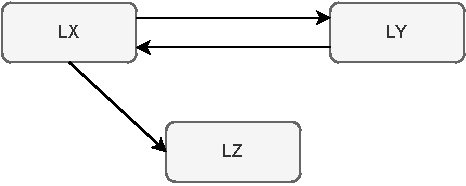
\includegraphics[width=0.6\textwidth]{\trainingsectiondir/figures/lxlylz.drawio}
\caption{Layered Architecture Example: Illustration of Two Top Layers (LX, LY) and a Bottom Layer (LZ).}
\label{fig:lxlylz}
\end{figure}

The objective of the bridge component is to enable the exchange of both \textbf{assets} and \textbf{messages} (See Figure \ref{fig:assets-messages}). On the one hand, the term \textbf{asset} refers to any digital representation of value within the Ethereum blockchain. Ethereum supports two types of assets: \textbf{Ether (ETH)}, which is the native cryptocurrency of the network, and \textbf{Tokens}, including ERC-20 and ERC-721 tokens. On the other hand, a \textbf{message} refers to communication or interaction between two smart contracts, involving both data and a value (in ETH) transferred from the origin contract (the one initiating the message) to the specified destination contract. Within the zkEVM context, these messages entail the execution of a function \texttt{onMessageReceived} of some existing contract. This is what we call the \textbf{messaging mechanism} of the bridge.

\vspace{1em}

\begin{figure}[H]
\centering
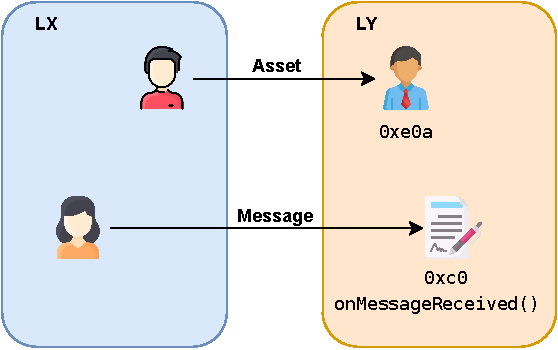
\includegraphics[width=0.4\textwidth]{\trainingsectiondir/figures/assets-messages.drawio}
\caption{The bridge component should be able to exchange both assets and messages.}
\label{fig:assets-messages}
\end{figure}

The core logic of the LXLY bridge is implemented in smart contracts. In particular, the main contract is called \texttt{zkEVMBridge.sol} that is deployed in any layer in which we want exchanging to be enabled. One of the design goals is that this smart contract \textbf{is exactly the same in all layers} (See Figure \ref{fig:bridge-claim-method}). This uniformity is intentional to maintain consistency in the logic whether exchanging assets or messages from a lower layer LY to an upper layer LX, or vice versa and hence externalizing the complexity associated with the layer position distinction from the core contract.

\vspace{1em}

\begin{figure}[H]
\centering
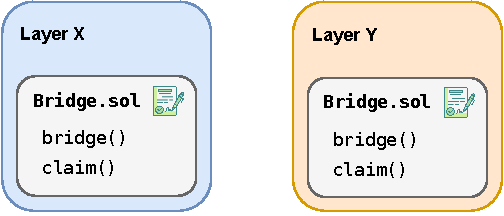
\includegraphics[width=0.5\textwidth]{\trainingsectiondir/figures/bridge-claim-method.drawio}
\caption{Uniform deployment of \texttt{zkEVMBridge.sol} in all layers ensures consistent handling of exchanges in the LXLY bridge's core logic.}
\label{fig:bridge-claim-method}
\end{figure}

The LXLY bridge follows a \textbf{bridge-claim model} (See Figure \ref{fig:lxly-exchange}). Let us suppose we are in the situation where some LX user want to transfer an asset (or, alternatively, a message) to some LY user. In the origin layer LX, the source user sends a transaction to the \texttt{bridge()} function providing the destination network LY. From now on, transactions to the bridge function will also be known as \textbf{deposits}. Later on, in the destination layer LY, the user sends a transaction to the \texttt{claim()} function providing the origin network LX in order to claim the \textit{transferred} (we will explore the meaning of that later on) asset (or message). To maintain a record of exchanges across layers, within the \texttt{zkEVMBridge.sol} smart contracts we need a compact way of storing the information of calls to the bridge function. These data, often referred to as \textbf{exits} or \textbf{outgoing transmissions}.

\vspace{1em}

\begin{figure}[H]
\centering
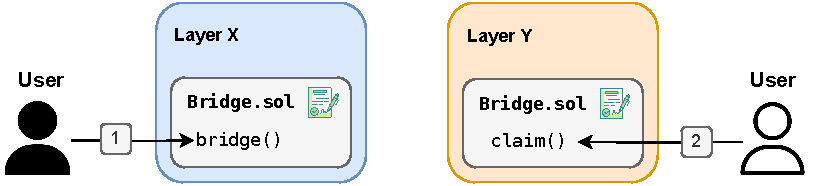
\includegraphics[width=0.7\textwidth]{\trainingsectiondir/figures/lxly-exchange.drawio}
\caption{LXLY bridge adopts a bridge-claim model for transferring assets and messages.}
\label{fig:lxly-exchange}
\end{figure}


\section{Exit Trees}

In order to store all the exits associated to a certain layer, the bridge contract builds an \textbf{append-only Merkle tree} having single exits, i.e., each call to the \texttt{bridge()} function, as its leaves. The Merkle tree with all the exits of a layer is called its \textbf{Local Exit Tree} (Figure \ref{fig:local-exit-tree}) and, its root is called \textbf{Local Exit Root (LER)}. It is important to remark that an exit tree is a different object and has a different structure than the tree that stores the L2 state.

\begin{figure}[H]
\centering
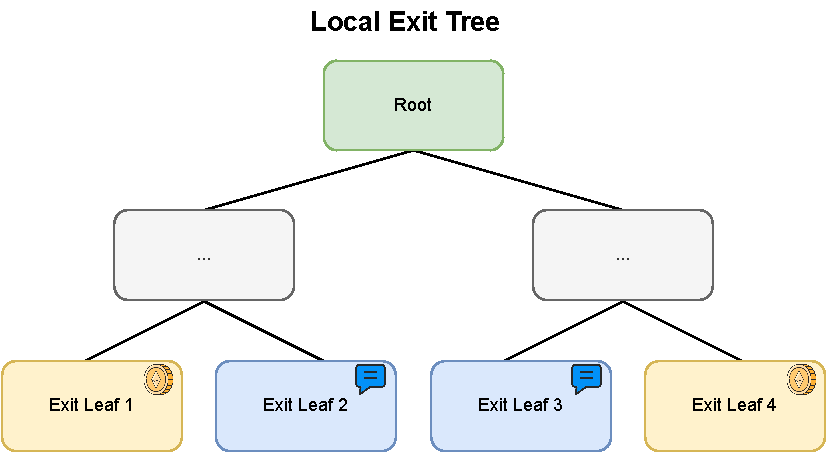
\includegraphics[width=0.6\textwidth]{\trainingsectiondir/figures/local-exit-tree.drawio}
\caption{Illustration of the Local Exit Tree containing $4$ exits (2 assets and 2 messages).}
\label{fig:local-exit-tree}
\end{figure}

The following listing provides a detailed breakdown of the data structure encapsulated within each leaf of a Local Exit Tree:

\vspace{1em}

\begin{solidity}
uint8 leafType,
uint32 originNetwork,
address originAddress,
uint32 destinationNetwork,
address destinationAddress,
uint256 amount,
bytes32 metadataHash
\end{solidity}

\begin{itemize}

\item \texttt{leafType}: This parameter serves as an identifier, distinguishing whether the leaf corresponds to an asset or a message. A value of $0$ designates an asset, while a value of $1$ signifies a message.

\item \texttt{originNetwork}: The identifier (\texttt{chainId}) of origin layer of the exchange.

\item \texttt{originAddress}: For asset exchanges, it represents the address of the token contract. For message exchanges, it denotes the source address of the bridge call.

\item \texttt{destinationNetwork}: The identifier of the destination layer (\texttt{chainId}) of the exchange.

\item  \texttt{destinationAddress}: Denotes the account receiving the asset or the address of the smart contract in the case of a message exchange.

\item  \texttt{leafAmount}: The amount of asset exchanged, encompassing both Ether or Tokens.

\item  \texttt{metadataHash}: This field captures the hash of the metadata associated with the exit. For asset exchanges, the metadata includes details such as the token's name, symbol, and decimals. Conversely, for message exchanges, the metadata comprises the calldata necessary for invoking the \texttt{onMessageReceived()} function, encapsulating the functional payload of the transmitted message.

\end{itemize}

In each layer, the corresponding bridge smart contract needs to be able to both \textbf{write} to and \textbf{read} from Local Exit Trees. On the one hand, the bridge contract will need to write in its Local Exit Tree each new exit resulting from a call to its \texttt{bridge()} function. On the other hand, the bridge contract needs to read the Exit Trees of other layers in order to process calls to the \texttt{claim()} function, since it should not be possible to claim something that has not been bridged, for example.

\begin{figure}[H]
\centering
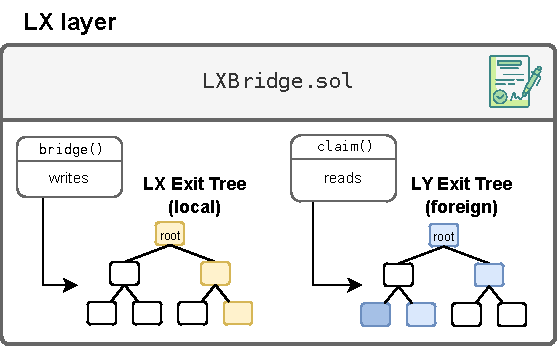
\includegraphics[width=0.4\textwidth]{\trainingsectiondir/figures/read-write-exit-trees.drawio}
\caption{Bridge contracts in each layer needs to both read and write to Local Exit Trees for a correct tracking within the bridge-claim model.}
\label{fig:rw-local-exit-tree}
\end{figure}

Moreover, in each layer, the corresponding bridge smart contract needs to additionally nullify the claim. Each claim must be locally nullified in
the bridge contract to avoid double claimings. The nullify process to avoid claiming transactions that have already been processed uses an efficient mapping
known as \texttt{claimedBitMap} (we will explain how this bitmap works later in more detail).

\begin{figure}[H]
\centering
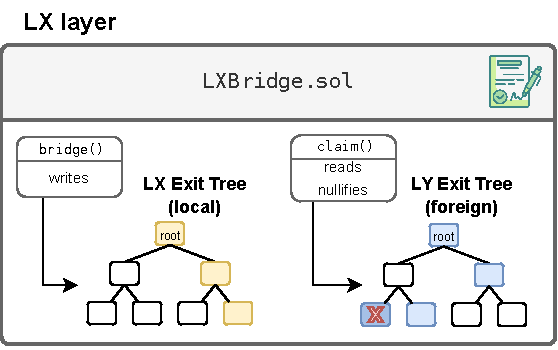
\includegraphics[width=0.4\textwidth]{\trainingsectiondir/figures/read-exit-trees-nullify.drawio}
\caption{Bridge contracts locally nullify claims to prevent duplicate claimings.}
\label{fig:nullify-claims}
\end{figure}

%TODO: Section explaining reads and nullifies.





% !TeX spellcheck = en_US
% !TeX root = ../build/communication-layer.tex
% !TeX TXS-program:compile = txs:///xelatex/[--shell-escape]


\section{Append Only Merkle Trees}

This section entails the design of an append-only sparse binary Merkle tree whose successive roots can be computed with a minimal amount of persistent data. This kind of trees are designed for scenarios where the tree represents an ordered list of data elements which can only be modified by appending new ones. Rather than storing the whole the tree, only two key elements are stored:

\begin{itemize}

\item An array of the size of the tree depth, denoted to as \texttt{branch}.

\item The last appended element's index, denoted to as \texttt{lastElementIndex}.

\end{itemize}


Importantly, the depth of the tree, representing its maximum capacity, is known a priori. This drops the necessity to use markers to distinguish between branches and leaves. Furthermore, note that the tree is inherently balanced.

By convention, for our append-only tree we are going to use $0$s as default value for empty leaves. Hence, when the list represented using theincremental Merkle tree is empty, the following holds:

\begin{align*}
h_i &= 0, \\
h_{j, k} &= h(0, 0) := h^{(00)}, \\
h_{m, n, l} &= h(h^{(00)}, h^{(00)}) := h^{(0000)}, \\
&\cdots
\end{align*}

Here, $h$ denotes the employed hash function, and the notation \texttt{,} signifies juxtaposition. Observe that, in this scenario, each of the hashes stored \textbf{do only depend on the level being stored}. Hence, we just need to compute a different hash value per level.

\paragraph*{A Toy Example}

For sake of simplicity, let’s consider as a toy example a small incremental Merkle tree of a maximum capacity of 8 leaves (hence, the having maximum depth of $d = \log_2(8) = 3$).





%\newpage
%\bibliographystyle{alpha}
%\bibliography{../bib/bibliography}

\newpage
\appendix

\end{document}